\section{Logistic Regression}
\noindent
{\color{LightRubineRed} \rule{\linewidth}{1mm} }

\subsection{Logistic Regression Problem} % (fold)
\label{sub:logistic_regression_problem}
% better than align* ?
\begin{gather*}
f(x) = \mathcal{P}(+1 | x ) \in [0,1]
\end{gather*}
% subsection logistic_regression_problem (end)
\subsection{Logistic Hypothesis} % (fold)
\label{sub:logistic_hypothesis}
\begin{align*}
h(x) &= \theta{(W^TX)} \\
     &= \frac{1}{1+\exp{(-W^TX)}} \\
\theta(s) &= \frac{1}{1+\exp{(-s)}}
\end{align*}
\textbf{Sigmoid}: smooth,monotonic \par
% subsection logistic_hypothesis (end)
\subsection{Three Linear Models}
\textbf{linear scoring function}: \par
\begin{gather*}
S = W^TX
\end{gather*}
\begin{center}
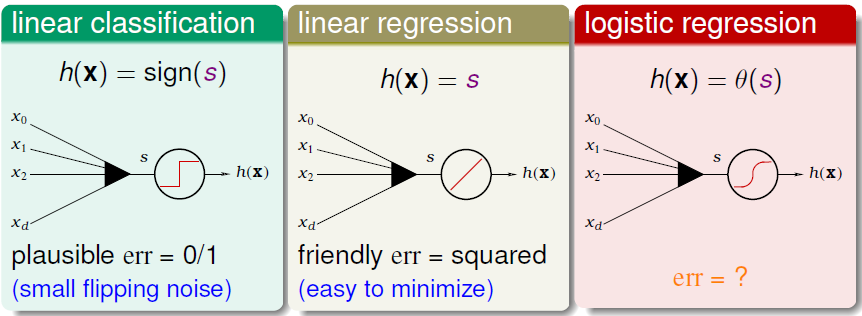
\includegraphics[width=14cm, height=5cm]{lecture10_1}\\
\end{center}
\textbf{Likelihood}
\begin{gather*}
\mathcal{P}(y|x) = 
\left\{  
             \begin{array}{lr}  
             f(x), &for \ y = + 1  \\  
             1- f(x), &for \ y= -1    
             \end{array}  
\right.  
\end{gather*}
\begin{align*}
 g^* &= \arg \underset{h}{max}\ \text{likelihood}(h) \\
 g^* & \propto \prod_{n=1}h(y_nx_n)
\end{align*}
\textbf{Cross-Entropy}
\begin{align*}
 \text{likelihood}{(w)} &\propto \underset{w}{\max} \prod \theta{(y_nW^Tx_n)} \\
 &\propto \underset{w}{\max} \log\prod\theta{(y_nW^Tx_n)} \\
 &\propto \underset{w}{\min} \sum - \log\theta{(y_nW^Tx_n)} \\
 &\propto \underset{w}{\min} \sum \log(1+\exp(-y_nW^Tx_n)) \\
 &\propto \underset{w}{\min} \sum \text{err}(W,x_n,y_n) \\
\end{align*}
 
\subsection{Minimizing $E_{in}(W)$}
用梯度链法求梯度就行了。 \par
求完梯度不像LR一样是close-form,一步登天。 \par
借鉴PLA思想iterative Optimization \par
\begin{align*}
w_{t+1} \gets w_t + \underbrace{1}_\eta \underbrace{\llbracket sign(w^Tx) \neq y_n\rrbracket * y_nx_n }_{\nu}
\end{align*}

\subsection{Gradient Descent}
尽管不能一次算出最好的$E_{in}$,可以用Greedy approch \par
\begin{align*}
W_{t+1} \gets W_t + \eta V \\
\underset{||v||=1}{\min} E_{in}(\underbrace{W_t+ \eta V}_{W_{t+1}})
\end{align*}
对于比较小的 $\eta$可以使用泰勒展开 
\begin{align*}
E_{in}(W_t+\eta V) \approx E_{in}(W_t) + \eta v^T \nabla E_{in}(W_t)
\end{align*}
要使$E_{in}(W_{t+1})$ 最小化,我们只需要保证$V$的方向和$\nabla$的\textcolor{mypink2}{方向相反}并且大小相同即可。(V即是W要走的方向)
\begin{align*}
V = -\frac{\nabla}{||\nabla||}
\end{align*}
\begin{myremark}{SGD}
\begin{align*}
W_{t+1} \gets W_t - \eta \frac{\nabla}{||\nabla||}  \\
\end{align*}
\end{myremark}
不同的$\eta$影响效果也不同,一个启发式的做法是根据梯度的模重新定义$\eta$ \par
\begin{center}
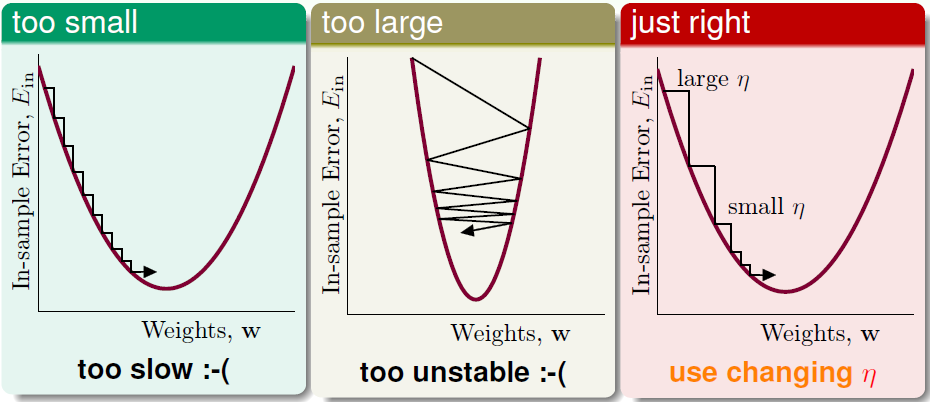
\includegraphics[width=14cm, height=5cm]{lecture10_2}\\
\end{center}
其实就是GD,算法不写了。
\begin{center}
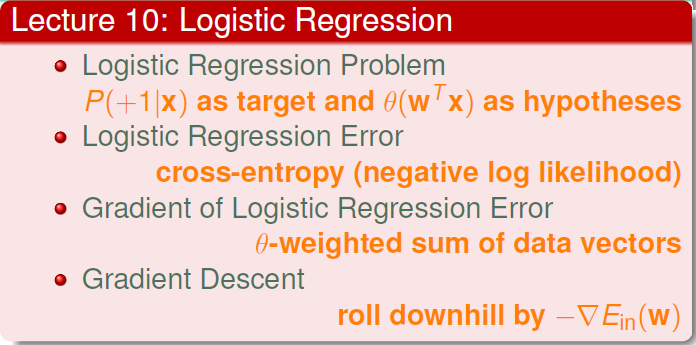
\includegraphics[width=10cm, height=5.5cm]{lecture10_sum}\\
\end{center}
\noindent
{\color{RubineRed} \rule{\linewidth}{1mm} }